\stopallthesefloats

\subsubsection{Unified WCET Analysis Framework}
\begin{figure}
\centering
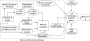
\includegraphics[width=\columnwidth]{\chapterdirectory/figure/handling_it/chattopadhyay_wcet.pdf}
\caption{%
Overview of the strategy presented in \cite{10.1145/2584654} (taken from the
paper)
}
\label{fig:handling_it:chattopadhyay}
\end{figure}
\cite{10.1145/2584654} presents a framework for WCET analysis on multi-core
platforms, which distinguishes itself from other solutions by the number of
features it takes into consideration. Indeed, the framework accounts for shared
caches, pipelines, and branch prediction. It also does not require the
assumption of a timing-anomaly-free architecture. An architecture free of
timing anomalies are architectures for which performing an operation faster on
a core cannot result in a longer execution time for the program compared to if
that operation took longer. The oppose would, for example, if the instruction
activates cache coherence mechanisms which would not have been necessary if the
in faster execution of that instruction. Readers interested in more possible
causes for timing anomalies are encouraged to read
\cite{DBLP:conf/wcet/ReinekeWTWPEB06}).
Figure~\ref{fig:handling_it:chattopadhyay} provides an overview of the
approach.  The assumptions that it does are as follow: use of a TDMA-based
round-robin arbitration policy, cores each have a private L1 cache. Data and
instructions are assumed to be fully separated (separate caches, separate
buses). Only instruction caches are taken into account (no cache coherence, no
possibility of modifications). Caches are assumed to be non-inclusive and to
use the LRU replacement policy.

The approach analyzes the WCET for each core separately.  Using abstract
interpretation, memory accesses are categorized according to whether they
always hit, always miss, or are marked as being unclassified. This is done for
both the L1 and L2 caches. The L2 cache can be a shared one, in which case
accesses susceptible to inter-core interference may move from always hits to
unclassified. This inter-core interference appears to be the only considered
direct interference from other cores, due to the assumptions made on the
architecture. Speculative execution, the result of branch prediction, may also
have effects on the contents of the L1 and L2 caches, as well as the pipeline's
behavior. A model of the shared bus's TDMA is taken into account when creating
the pipeline's model, adding a latency to certain stages. This pipeline model
creation process appears to be fairly complex, proceeding in an iterative
manner to compute the WCET of each basic computation block. Having the WCET of
each basic block, a model of the branch prediction mechanics and that of the
TDMA are used in the definition an linear optimization objective that will
return the WCET of the whole program.
